\chapter{Mechanisms of Polyspecificity}
\label{chap:chapter2}
\section{Introduction}
Human antibodies are critical for eradication of viral and bacterial infections, while providing the basis for immunological memory. Antibody protein molecules are encoded by several recombined germline gene segments prior to antigen exposure. The initial set of antibodies that are generated by recombination in the bone marrow is the antigen-na�ve antibody repertoire. It is of great interest to know how a finite set of such germline gene-encoded antibodies can recognize the large number of possible foreign antigens. A current hypothesis in the field suggests that antibodies encoded by germline gene segments are structurally flexible and therefore able to accommodate binding to many antigens, much like one glove fitting the shape of many hands. The phenomenon of one structure binding to many unrelated targets is known as polyspecificity. In this chapter, I will describe how I further support this hypothesis using computational design by showing the entire antibody protein variable region sequence is close to ideal for polyspecificity by mechanisms of flexibility. I will detail the computational protocol I have developed and the results that suggest how a finite set of antibody germline gene segments can encode antibodies that can engage a large number of potential antigens. Computational design of antibodies capable of binding multiple antigens may allow the rational design of antibodies that retain polyspecificity for diverse epitope binding, which will be an important to future vaccine design.

\subsection{Three Models of Protein Binding}
Antibodies are encoded by the rearrangement of variable (V), diversity (D), and joining (J) gene segments into recombined genes that encode a large but ultimately finite number of unmutated antibody structures, known as the germline repertoire \citep{Tonegawa:1983vw}. There are approximately 10$^{4}$ combinations of the V, D, and J heavy chain gene segments and an estimated 10$^{11}$ possible combinations when junctional diversity is considered \citep{Patten:1996vm}. This number of potential antibodies is far less than the immeasurable number of epitopes on foreign antigens to which one could be exposed. The germline gene repertoire therefore encodes a finite number of starting structures in the germline repertoire that must be capable of recognizing and binding a large and diverse array of antigens \citep{Patten:1996vm,Schultz:2002ef,Collins:2003wv}.

The classical protein binding mechanism was the "lock-and-key" model, where antibodies acquired somatic mutations in order to rigidify a pre-bound structure that would complement the shape of the epitope (figure \ref{fig:abmechanism}A). This mechanism dominated the field for many years but has to assume that one antibody optimally binds to one particular antigen \citep{Notkins:2004iz,James:2003ts}. The lock-and-key model has many shortcomings, as the "one paratope-one epitope" principle leaves little room to describe the polyspecificity phenomenon, an antibody's ability to recognize multiple unrelated antigens.

Polyspecificity has been demonstrated in a variety of biochemical and structural studies, therefore the "lock-and-key" model cannot possibly describe all antibody-antigen interactions without the existence of multiple paratopes per antibody \citep{Schultz:2002ef,Yin:2003wb,James:2003ip,Foote:1994tr}. In contrast to the "lock-and-key" model, a degree of pre-bound structural flexibility are found in two models of antigen binding, the "induced-fit" and the "conformational flexibility" models. In these models, germline gene-coded antibodies retain a degree of structural plasticity in their backbone in order to bind a number of different unrelated antigens. The induced-fit model hypothesizes that upon binding conformational changes are induced to accommodate the interacting structure (figure \ref{fig:abmechanism}B) \citep{Notkins:2004iz,James:2003ip}.

The conformational flexibility hypothesis in protein binding suggests that an unbound protein assume a variety of conformations (conformational isomerism), a subset of which is recognized by the interacting partner (figure \ref{fig:abmechanism}C). For antibodies, a large body of work has attributed polyspecificity to the nature of their germline gene sequences. It has been reported that polyspecific antibodies often retain a larger proportion of germline gene sequences than more mature, specific antibodies \citep{Notkins:2004iz,Chen:1991ug,Crouzier:1995ua,Harindranath:1993ty}.

\begin{figure}
   \centering
   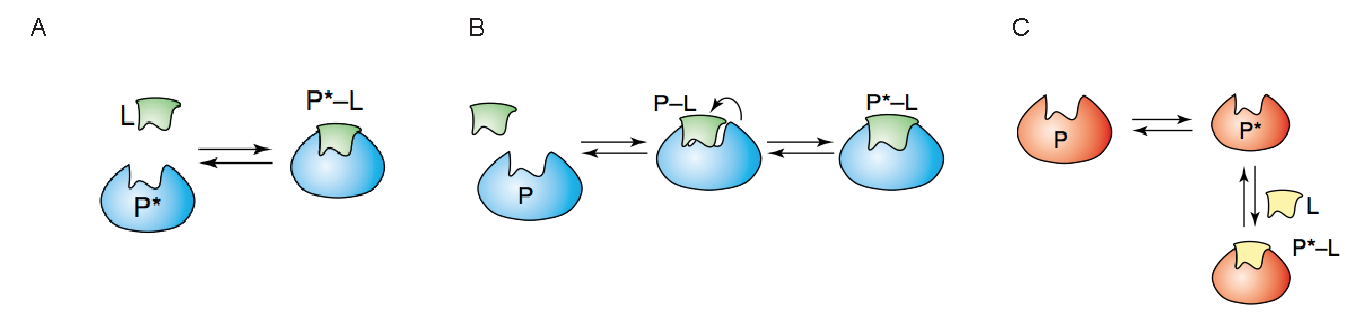
\includegraphics[width=1\textwidth]{images/chap2/figure2_1.pdf} %three modes of binding
   \caption[Three Models of Protein Binding]{ Three models of protein binding. The "lock-and-key" model assumes the protein binding site in a pre-bound state is optimized for the shape of the ligand (A). The "induced-fit" mechanism allows for conformational change after the ligand had bound to optimize shape in a two-step isomerization (B). For the "conformational flexibility" model, the pre-bound structure exists in several isomers which the ligand selects the conformation that complements it's structure (C). Figure adapted from \citep{James:2003ts} }
   \label{fig:abmechanism}
\end{figure}


\subsection{Evidence for Conformational Flexibility}
Conformational flexibility is emerging as an important hypothesis to explain both polyspecificity and changes in affinity between germline and mature antibody sequences \citep{Schultz:2002ef,Notkins:2004iz,James:2003ts,Yin:2003wb,James:2003ip,Foote:1994tr,Romesberg:1998ub,Manivel:2000wk,Yin:2001tq,Nair:2002wz,Jimenez:2003by,Li:2003ic,Mohan:2009hs,Marlow:2010jl,Wong:2011ff,Davies:1996wr,Mohan:2003ko,Wedemayer:1997wn,Zimmermann:2010fb}. The first evidence for conformational isomerism in antibodies was observed through kinetic experiments in which antibodies show a triphasic distribution that, in some cases, appears to reflect the existence of multiple isomers of the unbound antibody in solution, in the pre-equilibrium state \citep{James:2003ip}. To determine the dynamics of the binding process, James and colleagues examined the pre-steady-state kinetics of complex formation between SPE7 and DNP-Ser, as well as between SPE7 and the hapten cross-reactants. The kinetics confirmed the existence of an equilibrium in solution between two preexisting isomers, only one of which bound the haptens. Pre-steady-state binding kinetics were analyzed by monitoring changes in SPE7's intrinsic fluorescence upon rapid mixing with ligand.

In 1997, Wedemayer and colleagues found a structural basis for conformational flexibility observed for germline antibodies \citep{Wedemayer:1997wn}. They solved the crystal structures for a germline antibody with and without its target hapten, and mature antibody with six somatic mutations that bound the target hapten 30,000 times stronger than the germline counterpart. They noticed that the rigid-body deviation in the crystal structure was significant between the bound and unbound germline antibody structure indicating a degree of flexibility. In contrast, the mature antibody had less structural deviation upon hapten binding. They showed that the somatic mutations observed in the mature antibody stabilize the binding sites either directly or indirectly by locking the structure into the pre-bound conformation. This was the first indirect evidence showing that germline encoded antibodies may be more flexible than the mature sequences due to the intrinsic properties of the sequence.

More recently, structural studies along with computational tools have corroborated these findings by showing direct evidence that antibodies encoded by germline gene sequences retain flexibility in their HCDR3 loops \citep{Wong:2011ff,Babor:2009it}. For example, Babor \textit{et al.} redesigned germline or mature HCDR3 loops in antibodies that had been crystallized in free or antigen-bound states \citep{Babor:2009it}. These investigators found that germline gene-encoded HCDR3 sequences are nearly optimal for conformational flexibility. The study, while exceptional in its concept, was limited as the dataset contained many antibody/hapten (non-protein) complexes, which may not reflect the biology of interactions with larger protein targets that are more typical in foreign pathogens. Some antibodies classified as "germline" in the study were not from antigen-na�ve cells. Further, that study exclusively analyzed the HCDR3 loop, not the entire variable region.

Schmidt \textit{et al.} used molecular dynamics simulations and structural analysis to determine how mutations in the antibody variable domain enhance antigen binding to the influenza virus HA protein \citep{Schmidt:2013ka}. In the study, they found two broadly neutralizing antibodies that have branched in lineage from a common intermediate, and an unmutated common ancestor (UCA) in which they obtained high-resolution crystal structures. They found that even though the UCA and mature antibodies have nearly identical binding configurations, the affinity for influenza for the mature antibodies was 40-fold greater than the UCA. Molecular dynamics simulations predicted that the paratope in unbound UCA was not in an optimal conformation for binding, while the mature antibodies had a higher probability of being pre-configured for the influenza HA epitope.

\subsection{Experimental Rationale}
The V\textsubscript{H}-gene encodes the HCDR1, HCDR2, much of the immunoglobulin framework regions and the beginning of the HCDR3 loop. I hypothesized that the conformational flexibility mediating the polyspecificity of germline gene-encoded antibodies is determined at least in part by the heavy chain variable region encoded by the V\textsubscript{H}-gene, considering it makes up a large portion of the structure. The focus of my study was to test this hypothesis using computational design. Specifically, I analyzed the somatic mutations in sets of mature antibodies that derived from the same V\textsubscript{H} gene and for which co-crystal structures with biologically relevant target proteins were available. Sets of mature antibody-antigen complexes incorporating antibodies that derived from a common germline V\textsubscript{H}-gene were input into the \rosetta~"multi-state" design algorithm that recovers the optimal single sequence for an antibody to bind all antigens simultaneously \citep{Babor:2009it,Humphris:2007gq,LeaverFay:2011ji}. The sequences recovered using this protocol would be considered inherently flexible and polyspecific, since they are predicted to accommodate binding to diverse antigens using a structurally diverse set of antibody conformational states.
In contrast, I also tested monospecificity for each antibody by measuring which sequences are preferred during the design towards a single antigen. This is known as the "single-state" design protocol. For any change between the preference for sequence between the multi-state design protocol that considered polyspecificity and the single-state design that considers monospecificity, recapitulates \textit{in silico}, the process of affinity maturation.

Fundamentally, our approach compares germline and mature antibody sequences optimized in nature through evolution and maturation with sequences predicted to be optimal based on \rosetta's energy function applied to a set of co-crystallized antibody/antigen complexes. The power of the present approach is that I predicted germline and mature sequences \textit{in silico} without any prior knowledge of either, which is an important step towards rational antibody design. I would expect that results of this type of analysis will continue to improve as the size of the collection of conformational ensembles available in the Protein Data Bank (PDB) increases and as the accuracy of the \rosetta~energy function continues to improve.

\section{Multi- and Single-State Design of Antigen-Antibody Complexes}
I compiled panels of antigen-antibody complexes from the Protein Data Bank (PDB) in which the antibody heavy chain variable region were encoded by germline V\textsubscript{H}-genes, designated V\textsubscript{H}3-23, V\textsubscript{H}1-69, or V\textsubscript{H}5-51 \citep{Wu:2010dw,Tian:2008vq}. Antigen-antibody complexes were selected only if they contained Homo sapiens or humanized antibodies and the binding partner was a protein antigen. The search of the PDB returns 10, 8 or 3 candidate complexes for V\textsubscript{H}1-69, V\textsubscript{H}3-23, or V\textsubscript{H}5-51 respectively (table \ref{tab:dataset}).

\begin{table}[h]
\centering
\begin{tabular}{llllc}
\toprule
PDB ID & V\textsubscript{H}* Germline & Antibody    & Ligand    & V\textsubscript{H}* Mutations \\
\midrule
2CMR   & 1-69*01      & D5          & gp41      & 6             \\
3FKU   & 1-69*01      & F10         & HA        & 13            \\
3GBM   & 1-69*01      & CR6261      & HA        & 15            \\
3MA9   & 1-69*01      & 8066        & gp41      & 4             \\
3MAC   & 1-69*01      & 8062        & gp120     & 7             \\
3P30   & 1-69*01      & 1281        & gp41      & 20            \\
1G9M   & 1-69*02      & 17b         & gp120     & 21            \\
2DD8   & 1-69*05      & M396        & SARS-RBD  & 5             \\
2XRA   & 1-69*05      & HK20        & gp41      & 14            \\
2XTJ   & 1-69*10      & 1D05        & PCSK9     & 4             \\
2QQN   & 3-23*01      & anti-Nrps-1 & Nrps-1    & 10            \\
2R56   & 3-23*01      & IgE         & BLG       & 23            \\
2VYR   & 3-23*01      & VH9         & MDM4      & 10            \\
3KR3   & 3-23*01      & DX-2647     & IGF-II    & 8             \\
1S78   & 3-23*04      & Pertiuzimab & ErbB2     & 22            \\
2FJG   & 3-23*04      & G6          & VEGF      & 15            \\
3DVN   & 3-23*04      & Apu2.16     & Ubiquitin & 18            \\
3BN9   & 3-23*04      & E2          & MT-SP1    & 5             \\
2B1A   & 5-51*01      & 2219        & UG1033    & 17            \\
2XWT   & 5-51*01      & K1-70       & TSHR      & 8             \\
3HMX   & 5-51*01      & Ustekinumab & IL-12     & 12           \\
\bottomrule
\end{tabular}
\caption[Antibody-antigen test set]{Antibody-antigen test set. Details of the 10, 8, and 3 complexes for V\textsubscript{H}1-69, V\textsubscript{H}3-23, and V\textsubscript{H} 5-51 respectively. The antibodies bind a diverse set of antigens but each share a common germline across a test set. The V\textsubscript{H} mutation count of amino acid mutations away from their inferred germline gene. *Predicted from IMGT}
\label{tab:dataset}
\end{table}



For each panel I compared the mature (somatically mutated) sequence to the inferred germline gene sequence via a multiple sequence alignment (figure \ref{fig:polymethods}A). The number of mutations with respect to the germline sequence range from 4 to 23 mutations with an average of 12.2. All HCDR1, HCDR2, and framework positions that differed from the germline sequence of the common V\textsubscript{H}-gene sequence in at least one position in the multiple sequence alignment were included in the computational design simulations as "variable positions". Note that my study explicitly excluded positions that remained unchanged as no claims can be made with respect to the relevance of these positions for conformational flexibility or polyspecificity. My analysis is limited to antibody regions encoded by the V\textsubscript{H}-gene as only this region can be unambiguously aligned within each set of antibodies. Therefore, I excluded D-gene and J-gene that encode HCDRH3, and antibody light chain positions. The identity and conformation in all variable positions to identify the sequence and conformation that return minimal energy for the given protein backbone of the antibody/antigen complex \citep{Kuhlman:2000tc}. In this work, I used multi-state design \citep{LeaverFay:2011ji} to find a single sequence that minimized energy with all antigens within each V\textsubscript{H} gene-encoded group. To reduce noise in the outcome of the computations, 100 simulations were executed, and results are displayed using WebLogo representation \citep{Crooks:2004do} (figure \ref{fig:polymethods} C).

For a concrete example, consider position 31 (PDB numbering, boxed in \ref{fig:polymethods} C). This position, encoded by V\textsubscript{H}5-51, diverged from a germline serine residue in the sequence for all three complexes. Complexes 2B1A and 2XWT (PDB code) possess an aspartate residue in this position acquired by somatic mutation, while 3HMX has a threonine in the same position. The multi-state design protocol selected the germline residue serine as the energetically most favorable residue out of all 20 possible genetically encoded amino acids when interaction with all three structurally diverse antigens is required. The experiment was repeated as three separate "single-state design" experiments (figure \ref{fig:polymethods}B, right side) to predict the sequences and conformations that minimized interaction energy for each antigen individually. The resulting sequences were compared to both the inferred germline and the mature sequence (figure \ref{fig:polymethods}C). In this experiment position 31 is predicted as an aspartate for complexes 2B1A and 2XWT, and as a threonine for 3HMX, the mature amino acid sequence (data not shown).

For this work, it was important to convert the outcome to a statistical quantitative analysis. Each design outcome is compared to the mature or germline sequence, by computing a bit-score "recovery" measure. The results can either recover towards germline, mature or neither sequences. The bit-score computation I used is described in the methods of the appendix section. The advantage of the bit-score measure in comparison to a more simplistic percentage-recovery is that it analyzes the relative probabilities of all twenty amino acids in a particular sequence position, not just the probability of the correct one. It thereby arrives at an accurate measure of "surprise" of seeing a certain outcome, a normalized measure in information theory that can be readily compared between different experiments. In our experiment high bit-score for the germline sequence indicated that among the 100 designed sequences, germline gene-encoded residues were chosen in a large number of instances (figure \ref{fig:polymethods}D). To facilitate comparison across complexes that have a different number of designed entities considered, I determined the sum bit-scores over all designed positions and normalized the score to fall between 0 and 1 by division with the maximum bit-score that could be achieved, \textit{i.e.}, every amino acid position designed towards a germline or mature sequence.

\begin{figure}[t!]
\centering
 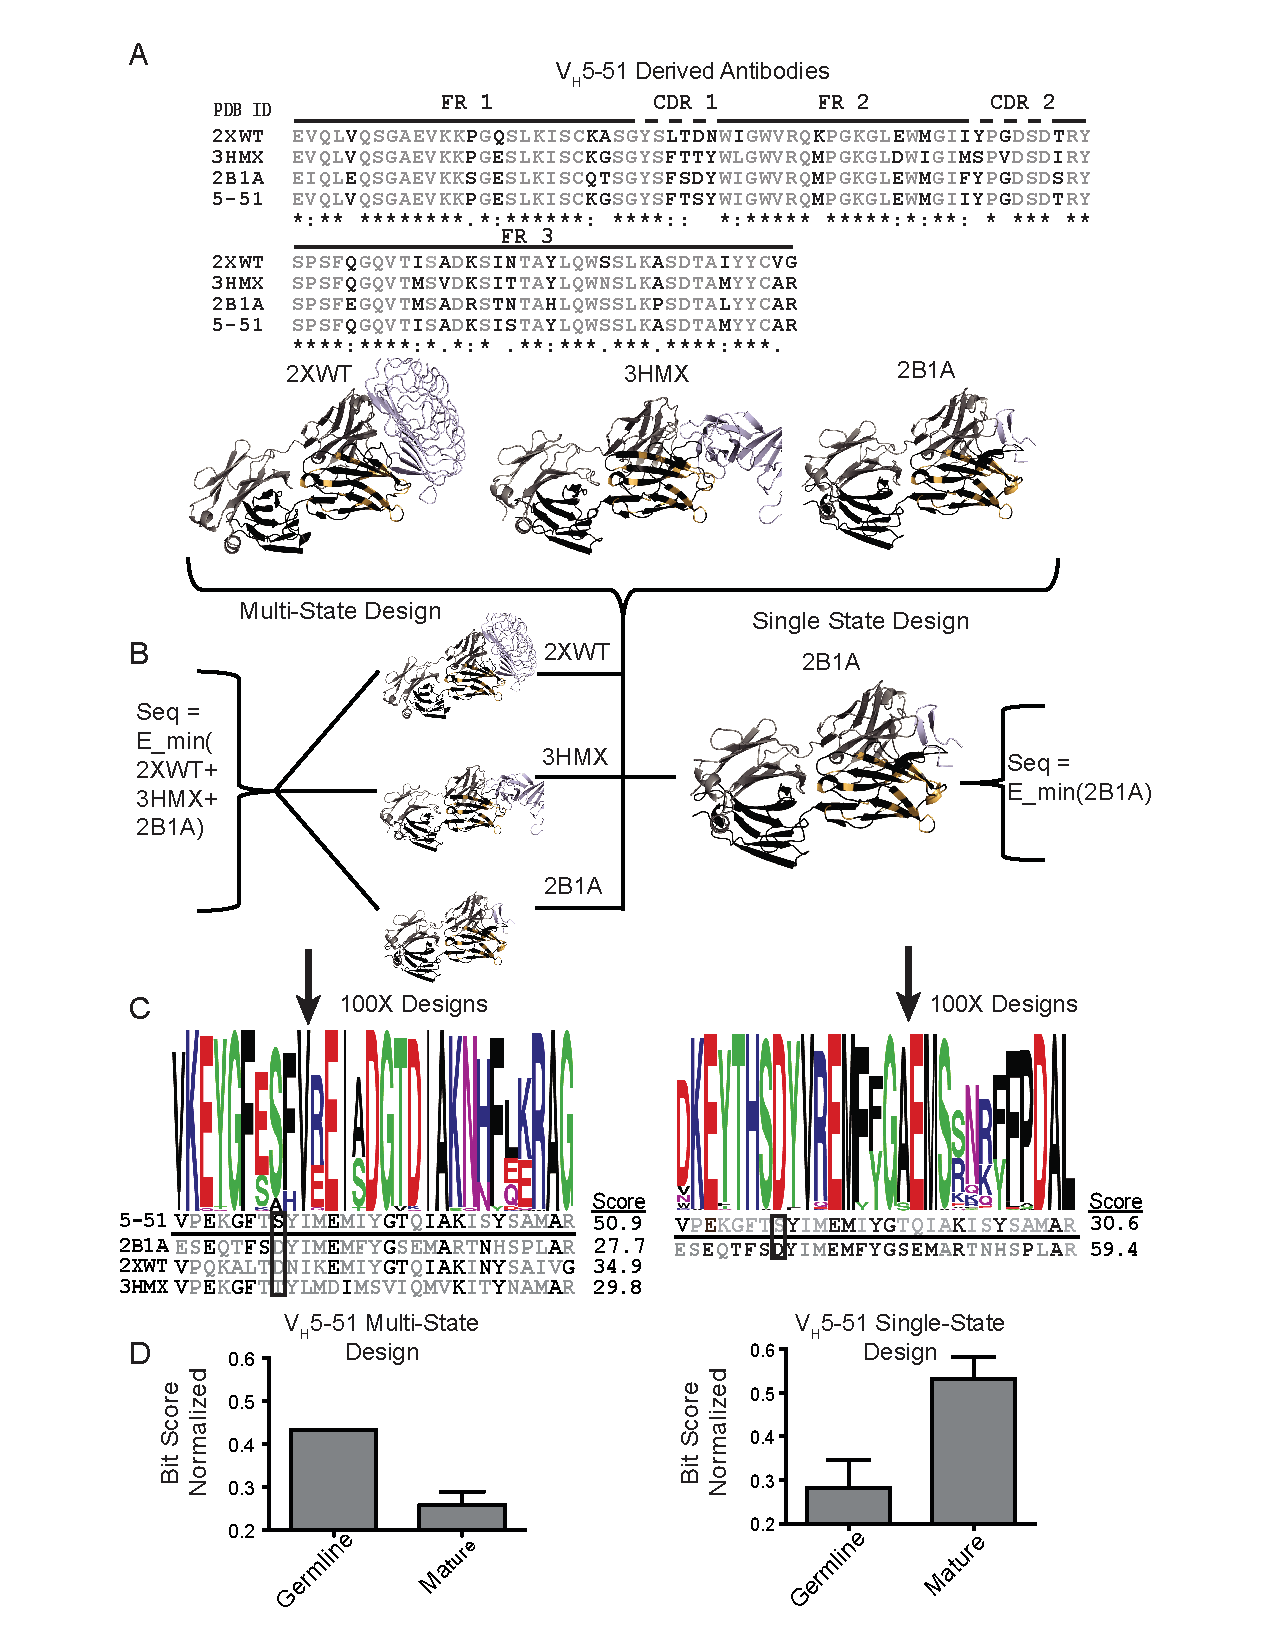
\includegraphics[width=.9\textwidth]{images/chap2/figure2_2.pdf}
   \caption[Multi-State and Single-State Design Methodology]{Multi-state and single-state design methodology. Position candidates were chosen for design if the position differed from the germline sequence in at least one mature complex (A). Co-crystal structures for each complex are shown with designed positions highlighted in gold. Single- and multi-state design schemes are shown (B)  Each position in the sequence logo corresponds to a position conserved for design (C). Bit-scores were determined quantitatively by measuring the frequency of a letter at each position (D).}
  \label{fig:polymethods}
\end{figure}



\section{Specificity Inferred by Sequence Design}
The results of the multi-state design simulations returned sequences that resembled germline gene-encoded sequences more often than mature sequences. This finding was remarkable as no information about germline sequences was input into the simulation. I found that the designed sequences gave normalized bit-scores of 0.54, 0.60, and 0.43 for germline genes V\textsubscript{H}1-69, V\textsubscript{H}3-23, or V\textsubscript{H}5-51, respectively. In contrast, statistically significant reduced bit-scores of 0.48, 0.45, or 0.26 (p < 0.0001) were observed when comparing the designed sequences with the mature genes (figure \ref{fig:polyresults}A).
The single-state redesign of mature antibodies for binding to their associated antigen gave normalized bit-scores of 0.47, 0.43, or 0.28 for comparison with germline gene-encoded sequences and 0.57, 0.54, or 0.53 for comparison with mature sequences of V\textsubscript{H}1-69, V\textsubscript{H}3-23 or V\textsubscript{H}5-51, respectively. In this design experiment, a proclivity to recover the somatically mutated mature sequences was observed (figure \ref{fig:polyresults}A). Given that a normalized bit-score is the preference for each design experiment to match a certain sequence profile, a high bit-score to germline sequence indicates the output matching the germline profile, while a high bit-score to the mature sequence indicates a preference for the mature profile, each design experiment outcome can be measured as a difference in bit-scores (mature - germline). With this definition, a preference for mature sequence gave a positive $\Delta$bit-score, while a preference for germline residues gave a negative $\Delta$bit-score for a given complex - \textit{i.e.}, the $\Delta$bit-score provided an \textit{in silico} predicted metric for antibody optimization for affinity to a specific antigen versus polyspecificty. I observed positive values for single-state design and negative values for multi-state design, indicating a preference for the mature or germline sequences, respectively (figure \ref{fig:polyresults}B, p < 0.0001).

\begin{SCfigure}
   \centering
   \caption[Multi-State Designs Toward the Germline Sequence ]{Multi-state designs toward the germline sequence. Antibodies encoded by the same inferred germline V\textsubscript{H} gene preferred germline sequences when considered in the multi-state design, inferring a more flexible combining site. The bar graph shows the bit-score for each of the three different inferred germline groups and then the sum of the scores in a grouped bar. A perfect design would have a normalized bit-score of 1.0, and summated score of 3.0 for three germline groups. Multi-state design preferred germline sequences for all complexes, while in contrast single-state design preferred mature sequences (A, p<0.0001). The change in bit-score is determined to be the proclivity to either the mature (positive score) or the germline (negative score) sequence. Each complex was assigned a change in bit-score. The change in proclivity between design protocols was significant (B, p< 0.0001). Each complex was scored against mature and germline sequences and a difference was calculated ($\Delta$bit-score). Positive numbers returned showed a proclivity towards mature sequences, while a negative score suggested a design toward germline. A tight correlation was observed (r$^{2}$=0.8263) for the \textit{in silico} predicted optimization for specificity versus polyspecificity ($\Delta$bit-score) and the \textit{in vivo} maturation process (C, plotted as the mutation percentage away from V\textsubscript{H} gene sequence).}
   	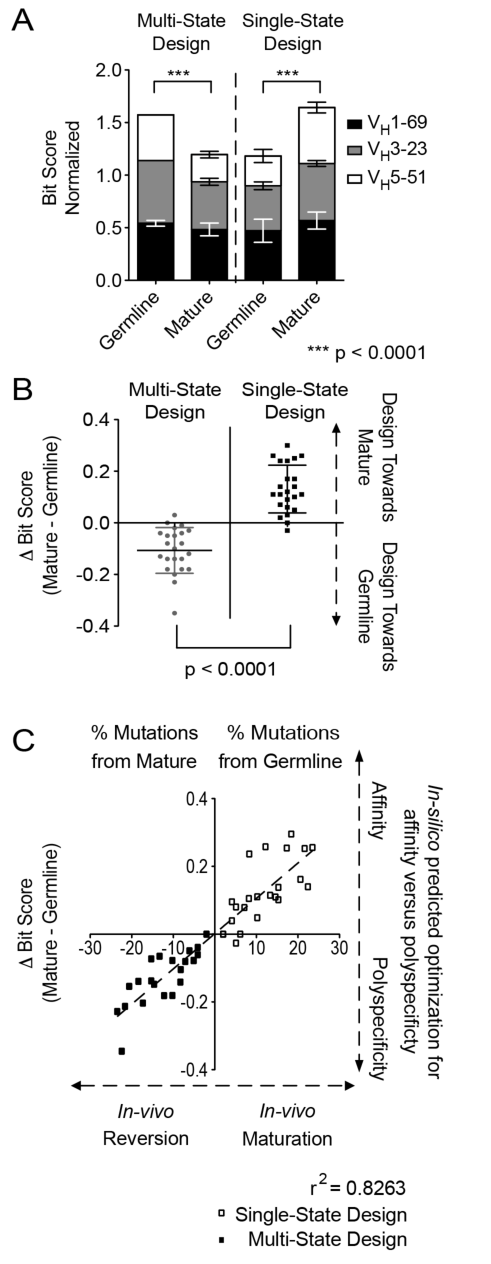
\includegraphics{images/chap2/figure2_3.pdf}
   \label{fig:polyresults}
\end{SCfigure}


\section{Affinity Maturation Correlates with Predicted Affinity}
The number of somatic mutations can be used as a measure of the maturity of an antibody \citep{Briney:2012ib}. Hence, I asked the question if the $\Delta$bit-score, the change in proclivity for a germline or mature sequence, correlated with affinity, \textit{i.e.}, if tendency to recover mature versus germline sequences increased as antibody maturation progressed. Such a correlation would indicate that as antibodies mature, features of the germline sequence critical for polyspecificity are replaced with features critical to recognize one target antigen. Figure \ref{fig:polyresults} C shows the somatic mutation percentage of antibodies in each complex as a metric  for ``\textit{in vivo} maturation'' correlated with the $\Delta$bit-score as a metric for "\textit{in silico} predicted optimization for affinity versus polyspecificty". For positive $\Delta$bit-scores, the mature sequence was preferred, indicating a preference for specificity. For negative values, the germline sequence, and hence polyspecificity was preferred. The correlation coefficient for the ``\textit{in vivo} affinity maturation'' and "\textit{in silico} predicted optimization for affinity vs. polyspecificity" was 0.83.

\section{Backbone Conformational Space for Germline Sequences}
Torsional phi-psi angles in the protein backbone were compared across the sets of experimental structures for positions that recovered to germline sequence for multi-state design and those positions that recovered to a non-germline sequence. I found that positions that converted back to germline in multi-state design, \textit{i.e.}, positions critical for conformational flexibility according to the simulation, had a deviation of 19.6$^\circ$ $\pm$ 2.0$^\circ$ across beta-sheet phi-psi torsion angles. Sequence positions that did not recover to a germline gene-encoded amino acid had a reduced deviation 15.5$^\circ$ $\pm$ 1.5$^\circ$ for beta-sheet backbone torsion angles (p = 0.099) (figure \ref{fig:polyfw} A-C). Considering the limited range for beta-sheet backbone torsion angles, I don't expect large deviations. For reference, all framework residue beta-sheets in antibody-antigen complexes across my dataset have an average phi-psi deviation of 18.7$^\circ$ $\pm$ 0.9$^\circ$.

\begin{SCfigure}
   \centering
   \caption[Phi-Psi Variances for Framework Residues]{Phi-psi variances for framework residues. The degree of structural variation of the framework residues were measured as the standard deviation of the phi and psi angles over each residue position. Side view of immunoglobulin fold for V\textsubscript{H}5-51 complexes aligned by framework residues. Beta-sheets included in the analysis are shown as a cartoon representation, while loop regions are in a transparent ribbon representation. Framework 1 is shown in brown, HCDR1 in green, framework 2 in black, HCDR 2 in magenta, and framework 3 in cyan (A). Same as (A) but top down view (B). The standard deviations of the phi-psi angles of each framework position were binned into either a residue that was found to be critical for polyspecificity (recovered to germline) or a residue that was not recovered to germline in multi-state design.  For each position, the phi-psi angles were averaged, and the standard error of the mean was calculated. An average of 19.6$^\circ$ $\pm$ 2.0$^\circ$ for germline recovered residues and 15.47$^\circ$ $\pm$ 1.5$^\circ$ for non-germline recovered residues supporting our hypothesis that residues which enable polyspecificity alter beta-sheet packing to a greater degree than residues that do not. The axis is normalized to 18.7$^\circ$ $\pm$ 0.9$^\circ$, the average deviation for all beta-sheet framework positions (C).}
   	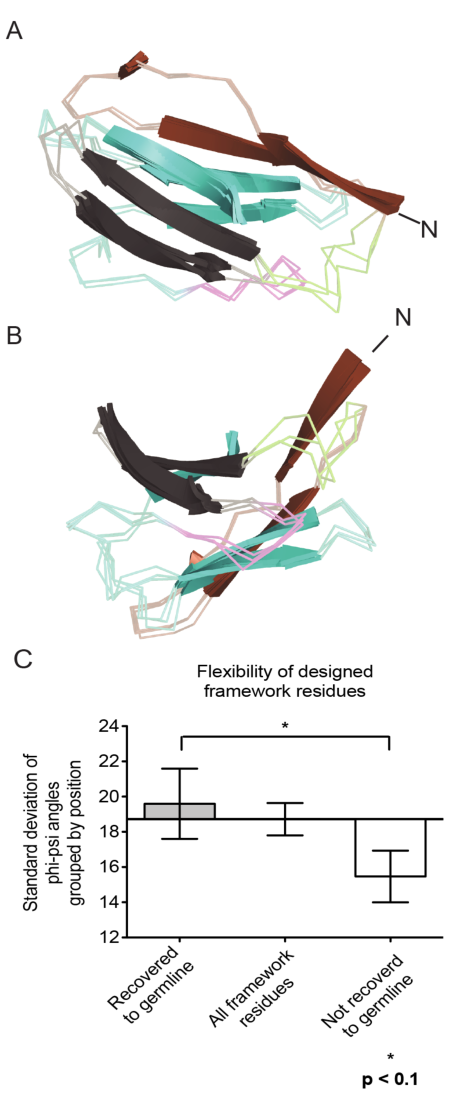
\includegraphics{images/chap2/figure2_4.pdf}
   \label{fig:polyfw}
\end{SCfigure}


\section{Impact of Residue Environment on Specificity}
Figure \ref{fig:polyenv} maps each amino acid position encoded by the V\textsubscript{H} gene segment onto the immunoglobulin fold using a custom Collier de Perles representation, as described by Ruiz and Lefranc \citep{Ruiz:2002jd}. I modified the output to distinguish positions by location in the interface with the antigen and the degree of burial. I correlated these metrics to the bit-score at a per-residue level. Each residue given is in IMGT numbering.

For multi-state design (figure \ref{fig:polyenv} A-C), 33 out of a possible 46 of the designed interface residues (72\%) contributed to polyspecificity, \textit{i.e.}, recovered to germline sequence with a normalized bit-score > 0. Remarkably, also 41 out of 77 residues outside the interface (53\%) recovered to germline. Residues 25, 40 and 105, far removed from the interface, recovered perfectly (normalized bit-score = 1) in at least two of the three germline gene test sets. These residues are highly buried, with a neighbor count score of 13.3 $\pm$ 0.5. The intermediately packed residues 17, 51, 70, and 71, with an average neighbor score of 8.6 $\pm$ 2.2 neighbors, were predicted to contribute to polyspecificity, even though they lie in distal positions from the antigen-binding site. The interface residues 35, 63, 64, and 82 were found to contribute to polyspecificity in two out of the three germline gene test sets. A conserved serine, which was found in all three germline sequences at position 36 in the CDR1, was the only residue identified as critical for polyspecificity in all three germline genes.

In contrast, for single-state design, it is more difficult to deduce overall trends for any specific position as the paratope is altered in each antibody and the recognized epitopes cover diverse structural space. Generally, when each complex was considered individually, 214 designed interface residues recovered to their mature sequence out of a possible 340 designed amino acids, indicating their importance for recognition of, and affinity for binding to, the specific antigen (63\%, figure \ref{fig:polyenv} D-F). When non-interface residues were considered, 411 out of a possible 699 designed residues recovered to their mature sequence (59\%).

Residues that were found to be critical for polyspecificity, \textit{i.e.}, reverted to germline in multi-state design, differed substantially for each germline gene test set considered. For the V\textsubscript{H}1-69 gene derived antibodies, all of the residues in the HCDR2 loop contributed to binding interactions in the single-state but not the multi-state design. In contrast only G63 and T64 residues contributed in the multi-state case but not in single-state designs. Residue L50 was recovered in all single-state complexes but was not critical for multi-state design. For the V\textsubscript{H}3-23 gene, residues A55 and Y66 were not recovered in multi-state design but were found to be important for high affinity in single-state design. For the V\textsubscript{H}5-51 complexes, non-interface residues P15, M53 and A80 were not recovered in multi-state design but were found to be critical in single-state design. HCDR2 was found to be critical in single-state design for all V\textsubscript{H}5-51 complexes.

\begin{figure}
\centering
 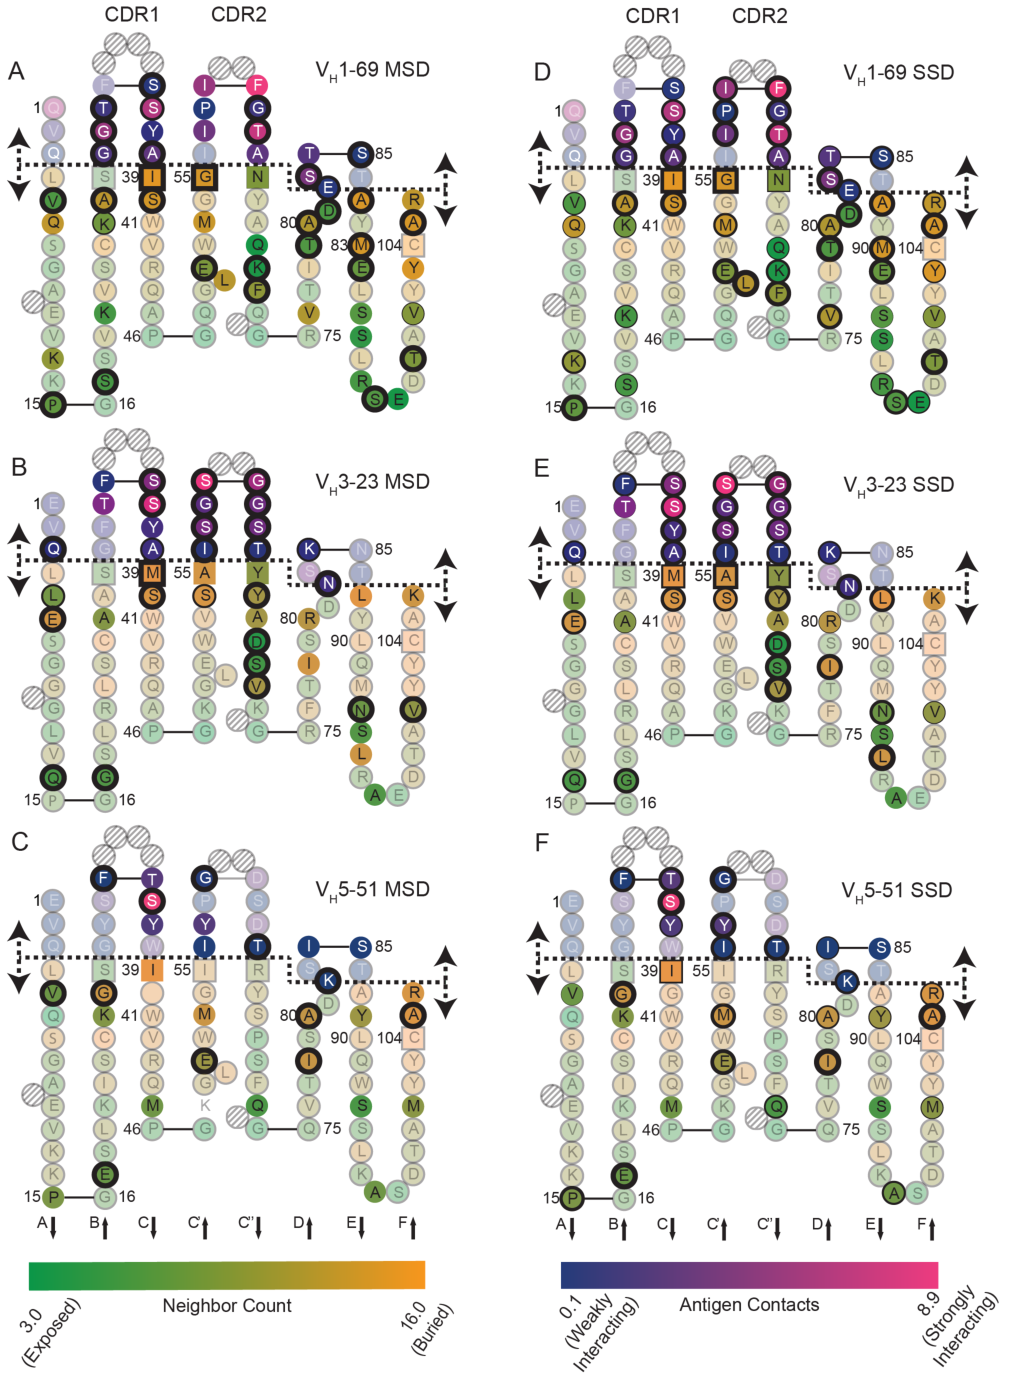
\includegraphics[scale=.7]{images/chap2/figure2_5.pdf}
   \caption[Colliers de Perles Representation of V\textsubscript{H} Gene Segments ]{Colliers de Perles reepresentation of V\textsubscript{H} gene segments. The 98 amino acids present in V\textsubscript{H}1-69, V\textsubscript{H}3-23, or V\textsubscript{H}5-51 are shown in a Collier de Perles two-dimensional representation and numbered according to the IMGT numbering scheme 37. Hatched circles are missing residues according to the IMGT numbering scheme and are shown to make graphs consistent. Square boxes represent the boundary between framework and CDR loops. A dashed line is shown for the interface. Interface residues are colored with a blue-pink gradient indicating a numerical antigen contact score defined by a change in neighbors between the free and bound complex. Non-interface residues are colored with a green-orange gradient according to their degree of burial defined through a neighbor count. A, B, C show the germline sequence represented in the immunoglobulin fold with the thickness of each line representing the design bit-score for that position relative to the germline sequence for multi-state design. D, E, F the thickness of the line corresponds to the mature sequence bit-score averaged over each complex.}
  \label{fig:polyenv}
\end{figure}


\section{Mature Sequence Bias}
\label{sec:maturebias}
To understand some of the trends described above more quantitatively, I determined for each residue in each antibody/antigen complex if it was part of the interface, \textit{i.e.}, directly engaging the antigen. For this purpose the change in neighbor count between unbound antibody and bound antibody/antigen complex score was measured, and positions with a change larger than 1.0 were classified as "interacting residues". Next, I counted how often a residue position appeared in the interface within each set of antibody/antigen complexes. Positions were binned as occurring in the ensemble interface never, once, two-four times, or more than four times and average bit-scores were compared (figure \ref{fig:polymsb}). I found a general trend for interface ensemble size correlating with interface ensembles sampled. For the set of structures derived from V\textsubscript{H}3-23, which contained a total of 8 complexes, I found that residue positions that are never found in the interface gave an average bit-score of 2.3 $\pm$ 0.4. If a residue position was found only in one interface, the average bit-score dropped to 1.2 $\pm$ 1.1. As residues were found more frequently at the interface between 2-4 complexes, and 5-8 complexes, the average bit-score increased to 2.5 $\pm$ 0.8 and 3.6 $\pm$ 0.7 respectively. For the 10 V\textsubscript{H}1-69 complexes, an average bit-score of 2.3 $\pm$ 0.3 was observed for residues that were never found in the interface. If a residue was only found in the interface once, the average bit-score dropped to 1.9 $\pm$ 1.0. For interface occurrences between 2-4 and 5-8, I found the average bit-score to increase to 2.6 $\pm$ 0.7 and drop to 0.8 $\pm$ 0.4 respectively. Due to the limited number of residues occurring in multiple interfaces, a significant change in bit-score between each grouping was not observed for V\textsubscript{H}1-69 (p= 0.1844) and V\textsubscript{H}3-23 residue positions (p=0.2007).

\begin{figure}[!t]
   \centering
   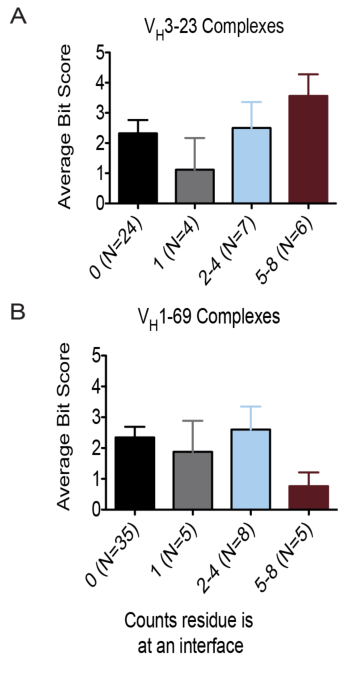
\includegraphics{images/chap2/figure2_6.pdf}
   \caption[Interface Occurrences Affect Germline Sequence Recovery]{Interface occurrences affect germline sequence recovery. For V\textsubscript{H}3-23 (A) and V\textsubscript{H}1-69 complexes (B), I binned each residue position into how many times it occurred in an interface (interface ensembles). Most designed positions never occurred in an interface. As their occurrences became more frequent, I observed a trend for increasing the recovered germline residue. This trend fell off for V\textsubscript{H}1-69 complexes (B) for positional occurrences between 5-8 interfaces.}
   	   \label{fig:polymsb}
\end{figure}


\section{Evolutionary Sequence Bias}
\label{sec:evobias}
I expected the result of multi-state design to deviate from germline in cases where alternate amino acids are compatible with the conformational space and binding modes observed in the ensemble of structures. Alternative amino acids might be tolerated but are not observed in evolution - "evolutionary sequence bias". To test this hypothesis, I reverted each position back to germline and compared the energetic change with the favored residue returned by multi-state design. Using reference energies, \rosetta~facilitates the direct comparison for energies between different residue types \citep{Kuhlman:2003kp}. For complexes derived from V\textsubscript{H}5-51, all positions in which the germline residue were not chosen in at least 10\% of the 100 simulated models were forced into the germline identity (figure \ref{fig:polyesb} A, x-axis). The difference in average energy of the germline sequence at that position from the average energy of the residue returned by multi-state design was calculated (y-axis). For each position, if positive values were returned for all three complexes, \rosettadesign~would most likely place a non-germline amino acid at that position. If negative values were returned for all three complexes, \rosetta~would most likely place a germline amino acid at that position. I found that, in most cases, the energetic contribution of the designed amino acid is not significantly more stabilizing than the germline amino acid, \textit{i.e.} the germline sequence is tolerated as well. Only positions 52, 76, 88, and 98 gave a significant energy increase for the germline sequence in at least one complex. Changes in energy were classified as significant if larger than 0.7 \rosetta~energy units (REU, horizontal dashed line). This threshold was derived from the average difference in energy between the germline and mature residue (0.7 $\pm$ 0.2 REU, data not shown). For Figure \ref{fig:polyesb}B, a multiple sequence alignment is given as a reference, where each position that was considered in multi-state design is highlighted in bold while each position that recovered well to the germline sequence is highlighted in green.

\begin{figure}[!t]
   \centering
   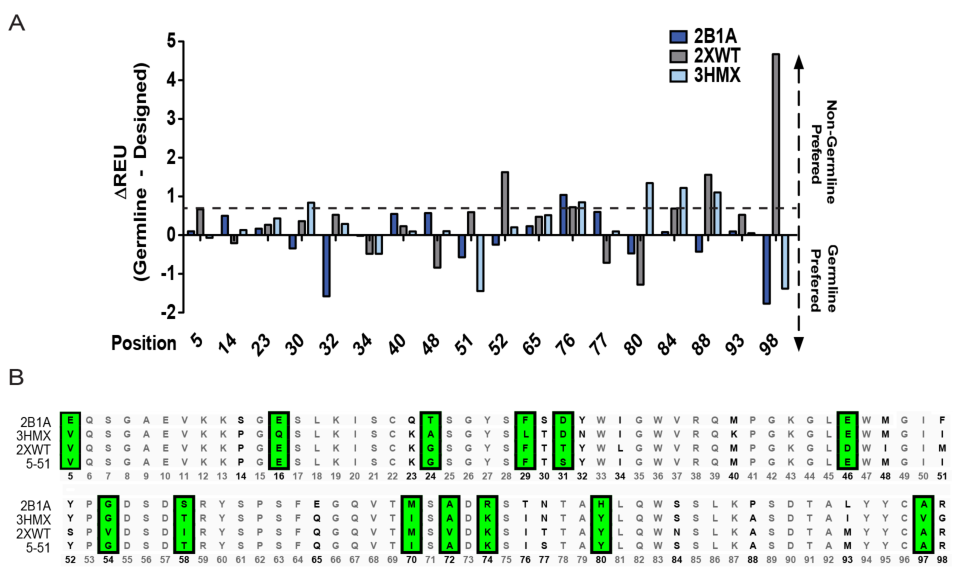
\includegraphics[width=\columnwidth]{images/chap2/figure2_7.pdf}
   \caption[\rosetta~Multi-State Design Solutions]{\rosetta~multi-state design solutions. I evaluated a complete germline reversion of V\textsubscript{H}5-51 sequence versus the sequences output by multi-state design. (A) Consideration of positions in which the multi-state design algorithm chose a non-germline amino acid for at least 10\% of the models where evaluated. The difference in energy of the germline sequence and the multi-state design solution sequence is shown for each position. Bars above 0 represent the multi-state design sequence preferred while bars below the line represent the germline amino acid preference. The horizontal dashed line at 0.7 \rosetta~energy units (REU) shows the average energy difference between the germline and mature sequence and is represented as a marker for sequence tolerance. (B) The multiple sequence alignment for each V\textsubscript{H}5-51 complex is shown and compared with the germline sequence. Sequences highlighted in bold were considered for design. Sequences highlighted in green are positions in which the multi-state design algorithm chose the germline amino acid as the design solution. The numbers in the bottom row are the alignment-numbering scheme of each position and correspond to the position numbers in (A).}
   	   \label{fig:polyesb}
\end{figure}



\section{Discussion}
\subsection{Limitations of Computation}
\label{sec:limits}
I recognize several important limitations of my study: \begin{enumerate}
\item I assumed that the \rosettadesign~protocol determined the optimal sequence for any given design challenge. While it has been demonstrated that \rosettadesign~typically recovers close-to-optimal sequences \citep{Kuhlman:2000tc}, inaccuracies in the scoring function and limitations in the sampling algorithm will introduce errors. In the future, this limitation could be reduced by improvements applied to the energy function and comparing the results obtained with complementary energy functions. I assumed that the finite and small set of antibody conformations observed in the set of co-crystallized mature antibodies completely describes the conformational flexibility of the germline gene-encoded antibody (finite ensemble bias). While I used the largest ensembles available (10, 8, and 3 antigen-antibody complexes), this assumption must be wrong, introducing a bias. For example, assume there is a sequence position that is part of the paratope in only one of the n complexes. In this antibody, a somatic mutation occurred at this position greatly increasing affinity to the antigen. The somatically mutated amino acid is however compatible with all other n-1 complex structures. In such a scenario the multi-state design algorithm will recover the somatically mutated instead of the germline amino acid. Here, I found that as a residue was more often part of the paratope, it became more likely to be recovered to the germline sequence. This finding might be due to the fact that a critical conformation that the germline antibody needs to adopt was not represented in the ensemble (for framework residues) or the epitope needed for recognition by a critical germline amino acid represented in the ensemble.

\item I assumed that the germline gene-encoded antibodies were able to adopt the conformations of each of the mature antibodies derived from it. This assumption is important, as crystal structures of the "true" germline antibody in complex with the antigen are generally not available. While this assumption is expected to be correct for the majority of cases, notable exceptions are discussed in the literature \citep{Yin:2003wb,Li:2003ic,Wedemayer:1997wn,Sethi:2006dq}.

\item It is not guaranteed that only the germline amino acid is compatible with all conformations adopted by mature antibodies. Rather, it is likely that for some positions alternative amino acids are plausible or even better in realizing the conformational flexibility needed. The germline sequence observed in nature is optimized in evolution and clearly works, but does not need to be perfect in all positions. In such a scenario, multi-state design could return amino acids that deviate from germline (evolutionary sequence bias). Conversely, the mature sequences observed in the co-crystal structures are not guaranteed to be the perfect sequence for high affinity. In some positions a somatic mutation might have introduced a better amino acid but is not the "true" best option. Some somatic mutations might have occurred by chance and do not contribute to affinity maturation. Some positions might not have experienced somatic mutations but still favorable mutations exist. In all these cases I expect the single-state design to deviate from the mature sequence observed in the co-crystal structure (evolutionary sequence bias).

\item The imperfect nature of the \rosetta~scoring function will not yield 100\% agreement with natural phenomenon \citep{Kuhlman:2000tc}. Importantly, water coordination can often be important in antibody-antigen binding sites. However, \rosetta~is currently being developed to include tools with explicit solvent models \citep{Lemmon:2012ku}.



\end{enumerate}
It is important to understand these biases and limitations to arrive at an accurate interpretation of the results. Given these known limitations, I expected imperfect agreement of \textit{in silico} predicted and natively observed mature and germline gene-encoded antibody sequences. Nevertheless, I found a remarkably high correspondence of residues designed for polyspecificity in a blinded fashion and the amino acids encoded by germline genes.

\subsection{Interpretation}
Germline gene-encoded sequences for commonly used V\textsubscript{H} segments are hypothesized to possess high conformational flexibility making them ideal for binding diverse antigens, \textit{i.e.}, being polyspecific. During antibody maturation, somatic mutations are introduced that increase affinity for a specific target in part by adding attractive interaction to the antigen (increasing enthalpic gain) and in part by locking the conformation critical for interaction with the specific antigen (reducing entropic cost). Here I tested this hypothesis by analyzing three sets of antibodies, each derived from a commonly used V\textsubscript{H} gene and each co-crystallized with a protein target in its antigen-specific binding conformation.

I chose to not directly compare conformational flexibility for germline and mature antibodies. While this approach may be feasible in general through predicting the accessible conformational space using molecular dynamics \citep{Wong:2011ff}, it is challenging to achieve complete sampling of large conformational spaces that include the entire immunoglobulin framework. To circumvent this problem, I chose to solve the inversely related protein design problem, which was to study amino acid sequences that are consistent with the conformational space seen in antibody/antigen co-crystal structures. This approach is complementary and potentially superior as it replaces sampling of the large conformational space in antibody backbone regions with solving the better understood ranking of amino acid sequences, given a certain antibody/antigen complex conformation. Specifically, I employed multi-state design to find single amino acid sequences that were compatible with the multiple conformations of antigen combining sites.

Computational tools to design multi-specific proteins were first described by pioneering work in the Kortemme laboratory \citep{Babor:2009it,Humphris:2007gq}. In parallel, Leaver-Fay and colleagues developed a general algorithm for multi-state design in the \rosetta~framework, in which they designed one protein to interact with non-native targets \citep{LeaverFay:2011ji}. I used the latter tool to design antibody sequences that are optimal for facilitating interactions to: \begin{enumerate}
\item Multiple and diverse antigens, or
\item A single specific antigen.
\end{enumerate}

In the absence of \textit{a priori} knowledge of the germline or mature sequences or the mechanism of antibody maturation through somatic mutations, multi-state design of one antibody to recognize several target proteins recovered sequences similar to those encoded by the inferred germline gene segment. When designing the same antibody to recognize one specific target, the sequence recapitulated the mature antibody sequence. This trend correlated tightly with the divergence of the mature sequence from the inferred germline sequence, \textit{i.e.}, the more somatic mutations an antibody contained, the more reversions to germline needed in order to facilitate interactions to multiple antigens.

Use of a computational tool to approach questions regarding polyspecificity as a function of protein sequence is advantageous, as the \rosettadesign~algorithm is able to rapidly enumerate the effect of multiple simultaneous mutations in sequence space for the entire heavy chain variable region. This task is quite difficult if not impossible to complete experimentally at this scale. In this manner, conformational flexibility in the framework regions, HCDR1, and HCDR2 can be tested in a holistic model. All mutated positions in the V\textsubscript{H} gene segment were considered simultaneously, including the effect of interactions between different domains in the antibody, thus revealing the role of interface and non-interface residues in both poly- and monospecificity. Because this approach considers multiple antibodies of variable conformation at once, each with a distinct binding mode, the multi-state design algorithm predicts sequences that are inherently flexible and capable of adopting the diverse set of conformations needed to bind to multiple antigens.

Harindranath and colleagues demonstrated that polyspecific antibodies were encoded largely by germline gene sequences \citep{Harindranath:1993ty}. Romesberg and Spiller presented structural evidence for flexibility in germline gene-encoded sequences \citep{Romesberg:1998ub}. In addition, Schmidt et al. correlated mature sequence to rigidity of the paratope \citep{Schmidt:2013ka}. Taken together, these data suggest conformational flexibility coupled with pre-sampled conformations of the target binding site as the underlying mechanism for polyspecificity \citep{Wedemayer:1997wn}. Here, I used a multi-state design algorithm to assess the contribution of the V\textsubscript{H} gene segment to specifying an antibody with conformational flexibility, preorganization, and polyspecificity. I found that this property is largely attributed to antibody sequences in the germline gene repertoire, since designing antibodies for polyspecificity, sequences recovered germline gene-encoded sequences, while designing antibodies for monospecificity to a single target, returned sequences similar to the mature antibody. This trend increased in strength the higher the number of somatic mutations that had accumulated, \textit{i.e.}, the further optimized the antibody had become. Importantly, the effect is not limited to the HCDR3, which often contributes much to antibody specificity. I obtained the same finding to be clearly measurable throughout HCDRs 1 and 2 as well as the immunoglobulin frameworks. I found each germline V\textsubscript{H} gene to encode a set of amino acids that enabled polyspecificity in a distinct manner. These positions were present not only in the paratope, but also in the buried or semi-buried positions of the immunoglobulin frameworks (figure \ref{fig:polyenv}). I expect, that with an increasing number of antibody-antigen complexes in the PDB it will become easier to discern general trends.

I conclude that conformational flexibility in the beta-sheet framework is critical for changing critical regulators of the conformation of the paratope - \textit{i.e.}, the takeoff and landing angles of HCDR loops, thereby enabling the paratope of germline antibodies to assume multiple conformations. Accordingly, I find that residues that contribute the most to polyspecificity contain larger deviations of their phi-psi torsion angles (figure \ref{fig:polyfw}). During antibody maturation, mutations in these positions likely lock in the target-specific framework conformation, reducing the entropic cost of target binding. Somatic mutations in the paratope, for example within HCDR1 and HCDR2, can directly increase affinity to a target (enthalpic contribution to free energy), or lock in a conformation that recognizes the target (entropic contribution to free energy). I found that on average 62\% of residues in the paratope and 42\% of residues in the framework were important for changing the binding pattern of the antibody from polyspecificity to recognition of one specific target (figure \ref{fig:polyenv}).

I identified at least four specific scenarios in which current datasets are limiting for informing design efforts:
\begin{description}

\item[The first scenario] involves a framework position that does not interact with the epitope in any of our tested complexes. For this position, the germline residue, and only the germline residue, is capable of adopting the phi-psi angles in order to accommodate the flexibility needed for the binding site. Multi-state design likely designs in the germline residue for each simulation. I then observe agreement between \textit{in silico} design and natively observed sequence for a majority of the designed positions (figure \ref{fig:polyresults}).

\item[The second scenario] involves a framework position that also lies distal from the epitope. In this scenario, the germline residue but also other amino acids are compatible with the observed conformations since they both contain properties to adopt the phi-psi angles necessary to accommodate the flexible binding site. For this scenario, I expect \rosetta's multi-state design algorithm to pick one of the compatible amino acids, not necessarily the germline gene-encoded one. This outcome can occur either because the conformational ensemble is incomplete or because of the evolutionary sequence bias. I find that both biases contribute to ambiguity. Residues that are never found in the interface give modest recovery to germline sequences being either "hit-or-miss" (finite ensemble bias, figure \ref{fig:polymsb}), and residues that are reverted to an amino acid different from that encoded in the germline are not significantly better in energy score than the germline encoded amino acid (evolutionary sequence bias, figure \ref{fig:polyesb})

\item[The third scenario] concerns residues that are at part of the paratope in only one instance. If the mature residue forms critical interactions that minimize the free energy of binding in this one complex, while in all other complexes the residue is not part of the paratope and the mature amino acid seen for the one complex is compatible with the backbone confirmation, \rosetta~will choose the mature residues from the first complex also in multi-state design mode. I observed this trend, especially for V\textsubscript{H}3-23 complexes. If a residue was found in only one interface (figure \ref{fig:polymsb}), that position tended to have a low recovery to the germline sequence.

\item[The last scenario] deals with positions that are part of the paratope multiple times and that experience frequent somatic mutations. As positions are found to be more frequently in interface ensembles, the germline recovery increases as these positions become more important to facilitating direct interactions with their antigen (figure \ref{fig:polymsb}). These residues contribute to polyspecificity by being the preferred residue in interaction with multiple antigens, rather than facilitating binding by altering beta-sheet packing.
\end{description}

\section{Conclusions and Future Directions}
These results suggest that the naturally occurring antibody maturation process can be recapitulated or reversed at least partially \textit{in silico}, opening exciting new avenues for antibody engineering work. Further, my results suggest the applicability of multi-state design to engineer polyspecific antibodies, exploring another important strategy for designing broadly neutralizing antibody therapeutics. Traditional antibody engineering approaches emphasize isolating monoclonal antibodies that are highly specific for a given antigen, relying on display techniques in which emphasis typically is placed only on HCDR loop design. The method described here considers the entire antibody variable region during design, including critical framework residues that allow for conformational flexibility and contribute to polyspecificity. Considering that I found that up to 64\% of framework and HCDR residues may contribute to binding and specificity, computational design will be invaluable to rapidly enumerate the large sequence and structural space of residues that can contribute to breadth of binding diverse targets.


